\section{p-n junctions and diodes}
\title{p-n junctions and diodes}  

\begin{frame}[plain]
    \titlepage
\end{frame}

%%%%%%%%%%%%%%%%%%%%%%%%%%%%%%%%%%%%%%%%%%%%%%%%%%%%%%%%%%%%%
%% Introduction to the p-n junctions %%
%%%%%%%%%%%%%%%%%%%%%%%%%%%%%%%%%%%%%%%%%%%%%%%%%%%%%%%%%%%%%
\begin{frame}
    \frametitle{What have you learnt and what you will learn?}

	\begin{itemize}
		\item WHat you have learnt so far? 
		\begin{itemize}
			\item How do a material behave as a conductor, semiconductor and insulator?
			\item How the current flows in a semiconductor?
			\item Mathematics of the current flow in a semiconductor?
			\item Proerpties of a intrinsic and extrinsic semiconductors?
			\item What is doping and \textbf{individual properties of n-type and p-type semiconductors?}
	\end{itemize}
		\item What you will learn in this lecture?
	\begin{itemize}
		\item What is a p-n junction? \textbf{How n-type and p-type semiconductors work together?}
		\item What is the depletion region?
		\item What is the built-in potential?
		\item What is the forward and reverse bias?
		\item What is the current-voltage characteristics of a diode?
		\item What are the different types of diodes?
		\item What are the applications of diodes?
	\end{itemize}
\end{itemize}
\end{frame}

%%%%%%%%%%%%%%%%%%%%%%%%%%%%%%%%%%%%%%%%%%%%%%%%%%%%%%%%%%%%%
%% Band diagrams of p-n junction %%
%%%%%%%%%%%%%%%%%%%%%%%%%%%%%%%%%%%%%%%%%%%%%%%%%%%%%%%%%%%%%
\begin{frame}
    \frametitle{Band diagrams of p-n junctions}
	\begin{itemize}
		\item A p-n junction is formed when a p-type semiconductor and an n-type semiconductor are brought into contact.
		\item The energy band diagrams of a p-n junction can be represented as follows:
		\begin{itemize}
			\item Before contact: The energy bands of the p-type and n-type semiconductors are separate.
			\item After contact: The energy bands of the p-n junction align, creating a depletion or space charge region at the interface.
			\item The conduction band and valence band of the n-type semiconductor are higher in energy than those of the p-type semiconductor.
			\item The Fermi level of the n-type semiconductor is higher than that of the p-type semiconductor before contact.
			\item After contact, the Fermi level becomes constant across the junction, indicating thermal equilibrium.
		\end{itemize}
		\item The energy band diagram of a p-n junction can be represented as follows:
\end{itemize}
\end{frame}


%%%%%%%%%%%%%%%%%%%%%%%%%%%%%%%%%%%%%%%%%%%%%%%%%%%%%%%%%%%%%
%% Band diagrams of p-n junction %%
%%%%%%%%%%%%%%%%%%%%%%%%%%%%%%%%%%%%%%%%%%%%%%%%%%%%%%%%%%%%%
\begin{frame}
    \frametitle{Band diagrams of p-n junctions}
	\begin{figure}
		\centering
		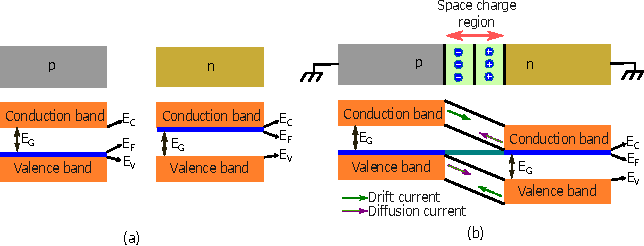
\includegraphics[width=0.8\textwidth]{fig/lec03/Band_diagram_all.pdf}
		\caption{Energy band diagram of a (a) discrete p and n (b) p-n junction.}
		\label{fig:pn_junction_all}
	\end{figure}
	\vspace{-0.5cm}
	\begin{itemize}
		\item The energy band diagram of a p-n junction shows the conduction band, valence band, and Fermi level of both the p-type and n-type semiconductors before and after contact.
		\item The depletion region is formed at the interface, where the majority carriers (holes in p-type and electrons in n-type) recombine, creating a region with no free charge carriers.
	\end{itemize}
\end{frame}


%%%%%%%%%%%%%%%%%%%%%%%%%%%%%%%%%%%%%%%%%%%%%%%%%%%%%%%%%%%%%
%% Band diagrams of p-n junction %%
%%%%%%%%%%%%%%%%%%%%%%%%%%%%%%%%%%%%%%%%%%%%%%%%%%%%%%%%%%%%%
\begin{frame}
	\frametitle{Band diagrams of p-n junctions}
	\begin{columns}
		\begin{column}{0.35\textwidth}
			\begin{itemize}
				\item \textbf{Step 1: Diffusion Due to Concentration Gradient}
				\begin{itemize}
					\item p-side: High hole concentration
					\item n-side: High electron concentration
					\item Result: Holes diffuse from p to n, electrons from n to p
				\end{itemize}
				\item \textbf{Step 2: Ions Left Behind → Space Charge}
				\begin{itemize}
					\item As mobile carriers leave, fixed ionized dopants remain:
					\begin{itemize}
						\item Negative acceptor ions in the p-region
						\item Positive donor ions in the n-region
					\end{itemize}
				\end{itemize}
			\end{itemize}
		\end{column}
		\begin{column}{0.7\textwidth}
			\begin{figure}
				\centering
				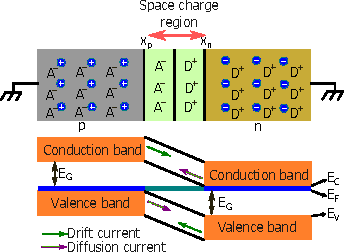
\includegraphics[scale=1.5]{fig/lec03/band_diagram_pn_junction_big.pdf}
				\caption{Energy band diagram of a p-n junction.}
				\label{fig:pn_junction}
			\end{figure}
		\end{column}
	\end{columns}
\end{frame}

%%%%%%%%%%%%%%%%%%%%%%%%%%%%%%%%%%%%%%%%%%%%%%%%%%%%%%%%%%%%%
%% Band diagrams of p-n junction %%
%%%%%%%%%%%%%%%%%%%%%%%%%%%%%%%%%%%%%%%%%%%%%%%%%%%%%%%%%%%%%
\begin{frame}
	\frametitle{Band diagrams of p-n junctions}
	\begin{columns}
		\begin{column}{0.5\textwidth}
			\begin{itemize}
				\item \textbf{Step 1: Diffusion Due to Concentration Gradient}
				\item \textbf{Step 2: Ions Left Behind → Space Charge}
				\begin{itemize}
					\item Creates a region with net charge — the \textbf{space charge region}
				\end{itemize}
				\item \textbf{Step 3: Built-in Electric Field Forms}
				\begin{itemize}
					\item The space charge generates an electric field $\mathcal{E}_{bi}$ (from n to p)
					\item This field opposes further carrier diffusion
				\end{itemize}
				\item \textbf{Step 4: Dynamic Balance Achieved}
				\begin{itemize}
					\item Eventually, drift current (due to $\mathcal{E}_{bi}$) balances diffusion current
					\item Net current = 0: system reaches \textbf{thermal equilibrium}
				\end{itemize}
			\end{itemize}
		\end{column}
		\begin{column}{0.5\textwidth}
			\begin{figure}
				\centering
				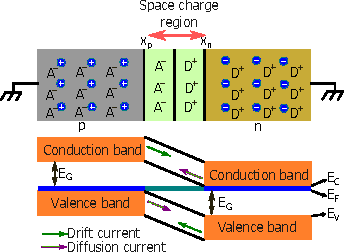
\includegraphics[scale=1]{fig/lec03/band_diagram_pn_junction_big.pdf}
				\caption{Energy band diagram of a p-n junction.}
				\label{fig:pn_junction}
			\end{figure}
		\end{column}
	\end{columns}
\end{frame}

%%%%%%%%%%%%%%%%%%%%%%%%%%%%%%%%%%%%%%%%%%%%%%%%%%%%%%%%%%%%%
%% Key insights in charge movement in p-n junctions %%
%%%%%%%%%%%%%%%%%%%%%%%%%%%%%%%%%%%%%%%%%%%%%%%%%%%%%%%%%%%%%
\begin{frame}
	\frametitle{Key Insights into Charge Movement}
	\begin{columns}
		\begin{column}{0.5\textwidth}
			\begin{itemize}
				\item Initial carrier flow is driven by \textbf{concentration gradients}, not electric forces.
				\item Opposite charges do not attract each other across the junction initially.
				\item The \textbf{electric field is a result of diffusion}, not the cause of it.
				\item The depletion region is characterized by:
				\begin{itemize}
					\item No free carriers
					\item Net space charge from fixed dopants
				\end{itemize}
				\item The system reaches an equilibrium defined by the \textbf{built-in potential} $V_{bi}$.
			\end{itemize}
		\end{column}
		\begin{column}{0.5\textwidth}
			\begin{figure}
				\centering
				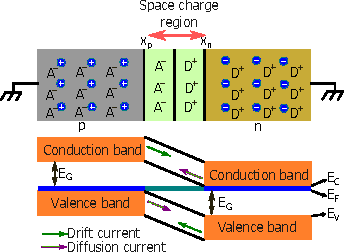
\includegraphics[scale=1]{fig/lec03/band_diagram_pn_junction_big.pdf}
				\caption{Energy band diagram of a p-n junction.}
				\label{fig:pn_junction}
			\end{figure}
		\end{column}
	\end{columns}
\end{frame}


%%%%%%%%%%%%%%%%%%%%%%%%%%%%%%%%%%%%%%%%%%%%%%%%%%%%%%%%%%%%%
%% Electric field intensity in space charge regions %%
%%%%%%%%%%%%%%%%%%%%%%%%%%%%%%%%%%%%%%%%%%%%%%%%%%%%%%%%%%%%%
\begin{frame}{Electric Field Intensity in the scpace charge region}
    \begin{itemize}
        \item The depletion region in a pn junction contains \textbf{uncompensated dopant ions} (donors in n-side, acceptors in p-side).
        \item This fixed charge distribution creates a \textbf{space-charge density} $\rho(x)$, giving rise to an electric field.
        \item According to \textbf{Poisson's equation}:
        \begin{equation}
            \frac{d^2 V}{dx^2} = -\frac{\rho(x)}{\varepsilon}
        \end{equation}
        where $V$ is the electrostatic potential and $\varepsilon$ is the permittivity.

        \item Integrating Poisson's equation yields the electric field:
        \begin{equation}
            \mathcal{E}(x) = \int_{x_p}^x \frac{\rho(x_n)}{\varepsilon} dx
        \end{equation}
        where $x_p$ is the reference point where $\mathcal{E}(x_p) = 0$.
    \end{itemize}
\end{frame}

%%%%%%%%%%%%%%%%%%%%%%%%%%%%%%%%%%%%%%%%%%%%%%%%%%%%%%%%%%%%%
%% Electric field intensity in space charge regions %%
%%%%%%%%%%%%%%%%%%%%%%%%%%%%%%%%%%%%%%%%%%%%%%%%%%%%%%%%%%%%%
\begin{frame}{Electric Field Intensity in the space charge region}
    \begin{itemize}
        \item \textbf{Electric field direction:}
        \begin{itemize}
            \item Points from n-side (positive charge) to p-side (negative charge).
            \item Corresponds to \textbf{negative field intensity} if potential decreases from n to p.
        \end{itemize}
        \item The electric field acts like an \textbf{internal dipole layer}, enabling the concept of \textbf{built-in potential} $V_0$.
		\item \textbf{Equilibrium condition:}
        \item At thermal equilibrium, i.e. the steady-state condition at a given temperature with no external excitations, the
		individual electron and hole currents flowing across the junctions are identically zero. Thus, for each type of
		carrier the drift current due to the electric field must exactly cancel the diffusion current due to the concentration
		gradient.
		\begin{equation}
			j_n = j_p = 0 \Rightarrow j_n + j_p = 0
		\end{equation}
		\item The total current density is given by:
		\begin{equation}
			j = j_n (\text{drift}) + j_p (\text{diffusion}) = q \left( \mu_n n \mathcal{E} + D_n \frac{dn}{dx} - \mu_p p \mathcal{E} - D_p \frac{dp}{dx} \right) = 0
		\end{equation}
    \end{itemize}
\end{frame}

%%%%%%%%%%%%%%%%%%%%%%%%%%%%%%%%%%%%%%%%%%%%%%%%%%%%%%%%%%%%%
% Built-in Voltage: Starting with Einstein Relation and Drift-Diffusion#
%%%%%%%%%%%%%%%%%%%%%%%%%%%%%%%%%%%%%%%%%%%%%%%%%%%%%%%%%%%%%
\begin{frame}{Built-in Voltage: Einstein Relation and Carrier Distribution}
    \begin{itemize}
        \item From the Einstein relation, the drift-diffusion equations become:
        \begin{align}
            j_n &= q \mu_n \left( n \mathcal{E} + \frac{kT}{q} \frac{dn}{dx} \right)  \\
            j_p &= q \mu_p \left( p \mathcal{E} - \frac{kT}{q} \frac{dp}{dx} \right) 
        \end{align}
        \item At equilibrium ($j_p = 0$), using integration of the expression inside the bracket gives:
        \begin{equation}
            p(x) = p(x_p) e^{-\frac{qV(x)}{kT}}
        \end{equation}
        \item With $V(x) = - \int_{x_p}^{x} \mathcal{E}(x') dx'$
        \item Similarly for electrons:
        \begin{equation}
            n(x) = n(x_n) e^{\frac{qV(x)}{kT}} 
        \end{equation}
        \item These distributions are referred to as the \textbf{Boltzmann distribution} under equilibrium.
    \end{itemize}
\end{frame}

%%%%%%%%%%%%%%%%%%%%%%%%%%%%%%%%%%%%%%%%%%%%%%%%%%%%%%%%%%%%%
% Built-in Potential Derivation
%%%%%%%%%%%%%%%%%%%%%%%%%%%%%%%%%%%%%%%%%%%%%%%%%%%%%%%%%%%%%
\begin{frame}{Derivation of Built-in Potential $V_{bi}$}
    \begin{itemize}
        \item Carrier product at any point:
        \begin{equation}
            n \cdot p = n_i^2 
        \end{equation}
        \item Built-in potential is given by:
        \begin{equation}
            V_{bi} = V(x_n) = \frac{kT}{q} \ln\left( \frac{p(x_p)}{p(x_n)} \right) = \frac{kT}{q} \ln\left( \frac{p(x_p) \cdot n(x_n)}{n_i^2} \right) 
        \end{equation}
        \item Assuming complete ionization at boundaries:
        \begin{equation}
            V_{bi} \cong \frac{kT}{q} \ln\left( \frac{N_A(x_p) \cdot N_D(x_n)}{n_i^2} \right) 
        \end{equation}
        \item This shows that $V_{bi}$ depends only on the doping levels and intrinsic carrier concentration.
        \item Important for setting the electrostatic barrier preventing further diffusion across the junction.
    \end{itemize}
\end{frame}

%%%%%%%%%%%%%%%%%%%%%%%%%%%%%%%%%%%%%%%%%%%%%%%%%%%%%%%%%%%%%
% Summary and insights in built-in potential
%%%%%%%%%%%%%%%%%%%%%%%%%%%%%%%%%%%%%%%%%%%%%%%%%%%%%%%%%%%%%
\begin{frame}{Key Insights from Built-in Potential Derivation}
    \begin{itemize}
		\item \textbf{1. Drift-Diffusion Balance at Equilibrium}
		\begin{itemize}
			\item Currents consist of drift + diffusion components.
			\item At equilibrium: $j_n = j_p = 0 \Rightarrow$ drift current = $-$ diffusion current.
		\end{itemize}

        \item \textbf{2. Carrier Densities Follow Boltzmann Distributions}
        \begin{itemize}
            \item $p(x) = p(x_p) e^{-\frac{qV(x)}{kT}},\quad n(x) = n(x_n) e^{\frac{qV(x)}{kT}}$
            \item Potential $V(x)$ governs spatial variation in carrier concentration.
        \end{itemize}

        \item \textbf{3. Mass Action Law Holds:} $n(x) \cdot p(x) = n_i^2$ \textit{everywhere in depletion region}

        \item \textbf{4. Built-in Voltage Expression:}
        \begin{equation}
            V_{bi} = \frac{kT}{q} \ln\left(\frac{N_A(x_p) \cdot N_D(x_n)}{n_i^2}\right)
		\end{equation}
        \begin{itemize}
            \item Depends only on doping densities and intrinsic carrier concentration.
            \item Sets up internal electrostatic barrier to prevent further diffusion.
        \end{itemize}

        \item \textbf{5. Interpretation:}
        \begin{itemize}
            \item \textit{Defines equilibrium energy band bending and barrier height.}
            \item \textit{Logarithmic dependence allows efficient doping control of $V_{bi}$.}
        \end{itemize}
    \end{itemize}
\end{frame}


%%%%%%%%%%%%%%%%%%%%%%%%%%%%%%%%%%%%%%%%%%%%%%%%%%%%%%%%%%%%%
% Biasing of p-n junctions
%%%%%%%%%%%%%%%%%%%%%%%%%%%%%%%%%%%%%%%%%%%%%%%%%%%%%%%%%%%%%
\begin{frame}{Biasing of p-n junctions}
	\textbf{All discussions in the previous slides were based on the assumption of thermal equilibrium and no external fields.} \\
	The behavior of a p-n junction can be controlled by applying an external voltage across the junction. This is known as \textbf{biasing}. \\
	\textbf{Biasing} refers to the application of an external voltage across a p-n junction to control its operation. The two main types of biasing are:
	\begin{columns}
		\begin{column}{0.5\textwidth}
			\begin{itemize}
				\item \textbf{Forward Bias:} Positive voltage applied to the p-side and negative voltage to the n-side.
			\end{itemize}
			\begin{figure}
				\centering
				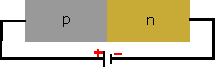
\includegraphics[scale=1]{fig/lec03/pn_forward_bias.pdf}
				\caption{Forward bias of a p-n junction.}
				\label{fig:forward_bias_pn_junction}
			\end{figure}
		\end{column}
		\begin{column}{0.5\textwidth}
			\begin{itemize}
				\item \textbf{Reverse Bias:} Positive voltage applied to the n-side and negative voltage to the p-side.
			\end{itemize}
			\begin{figure}
				\centering
				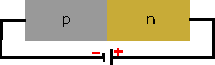
\includegraphics[scale=1]{fig/lec03/pn_reverse_bias.pdf}
				\caption{Reverse bias of a p-n junction.}
				\label{fig:reverse_bias_pn_junction}
			\end{figure}
		\end{column}
	\end{columns}
\end{frame}

\begin{frame}{Reverse bias in a \textit{p-n} Junction}
    \textbf{Key Concept:} Reverse bias widens the depletion region and blocks majority carrier flow.
    \begin{itemize}
        \item \textbf{Biasing:} Negative terminal to $p$-side, positive to $n$-side (Fig. 3-2a).
        \item \textbf{Effect:} Drives majority carriers (holes in $p$, electrons in $n$) \textit{away} from the junction.
        \item \textbf{Depletion Region:} Widens due to carrier drift, increasing the electric field barrier.
        \item \textbf{Steady State:} Cannot sustain continuous diffusion without replenishment $\Rightarrow$ nominally zero current.
        \item \textbf{Reverse Saturation Current $I_0$:}
        \begin{itemize}
            \item Small current due to minority carriers thermally generated.
            \item $I_0$ increases with temperature, but is \textit{independent} of applied reverse voltage.
        \end{itemize}
        \item \textbf{Physical Insight:} Potential barrier increases by $qV \Rightarrow$ blocks majority carriers, but allows minority carriers to flow.
		\item \textbf{Reverse Bias Breakdown:} If reverse voltage exceeds a critical value, breakdown occurs (Zener or avalanche breakdown).
    \end{itemize}
\end{frame}

\begin{frame}{Forward bias in a \textit{p-n} Junction}
	\begin{columns}
		\begin{column}{0.7\textwidth}
			\textbf{Key Concept:} Forward bias lowers the potential barrier and allows majority carrier injection.
			\begin{itemize}
				\item \textbf{Biasing:} Positive terminal to $p$-side, negative to $n$-side.
				\item \textbf{Effect:} Lowers the junction barrier height by $qV$, aiding carrier diffusion.
				\item \textbf{Depletion Region:} Narrows, reducing the internal electric field.
				\item \textbf{Carrier Movement:}
				\begin{itemize}
					\item Holes from $p$ move into $n$-side $\Rightarrow$ \textit{injected minority current}
					\item Electrons from $n$ move into $p$-side $\Rightarrow$ \textit{minority current in opposite direction}
				\end{itemize}
				\item \textbf{Current Flow:} Resultant current = sum of hole and electron minority currents.
				\item \textbf{Diode Equation:} $I = I_0 \left(e^{qV/kT} - 1\right)$ (derived later)
    	\end{itemize}
	\end{column}
		\begin{column}{0.3\textwidth}
			\begin{figure}
				\centering
				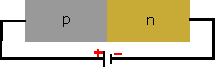
\includegraphics[scale=1]{fig/lec03/pn_forward_bias.pdf}
				\caption{Forward bias of a p-n junction.}
				\label{fig:forward_bias_pn_junction}
			\end{figure}
		\end{column}
	\end{columns}
\end{frame}